\documentclass[11pt]{article}

\usepackage{amsmath, amssymb, amsthm}
\usepackage{tikz}

\theoremstyle{plain}
\newtheorem{thm}{Theorem}[section]
\newtheorem*{thm*}{Theorem}
\newtheorem{prop}[thm]{Proposition}
\newtheorem{lem}[thm]{Lemma}
\newtheorem*{lem*}{Lemma}
\newtheorem{dfn}[thm]{Definition}
\newtheorem{cor}[thm]{Corollary}
\newtheorem{claim}[thm]{Claim}
\newtheorem{conj}[thm]{Conjecture}
\newtheorem{ques}[thm]{Question}
\newtheorem*{rem}{Remark}


\oddsidemargin  0pt
\evensidemargin 0pt
\marginparwidth 40pt
\marginparsep 10pt
\topmargin 0pt
\headsep 10pt
\textheight 8.2in
\textwidth 6.4in
\renewcommand{\baselinestretch}{1.1}

\newcommand{\codeg}{\text{codeg}}
\newcommand{\BBE}{\mathbb{E}}
\newcommand{\BFP}{\mathbf{P}}
\usepackage{amsmath}
\usepackage{amsthm}
\usepackage{amssymb}
\usepackage{mathtools}
\usepackage{hyperref}
\usepackage{url}





\usepackage{graphicx}
\usepackage{caption}
\usepackage{subcaption}

\def\eQb#1\eQe{\begin{eqnarray*}#1\end{eqnarray*}}
\def\eQnb#1\eQne{\begin{eqnarray}#1\end{eqnarray}}
\providecommand{\e}[1]{\ensuremath{\times 10^{#1}}}
\providecommand{\pb}[0]{\pagebreak}
\DeclarePairedDelimiter\ceil{\lceil}{\rceil}
\DeclarePairedDelimiter\floor{\lfloor}{\rfloor}

\newcommand{\E}{\mathrm{E}}
\newcommand{\Var}{\mathrm{Var}}
\newcommand{\Cov}{\mathrm{Cov}}

\def\Qb#1\Qe{\begin{question}#1\end{question}}
\def\Sb#1\Se{\begin{solution}#1\end{solution}}


\newtheoremstyle{quest}{\topsep}{\topsep}{}{}{\bfseries}{}{ }{\thmname{#1}\thmnote{ #3}.}
\theoremstyle{quest}
\newtheorem*{definition}{Definition}
\newtheorem*{theorem}{Theorem}
\newtheorem*{lemma}{Lemma}
\newtheorem*{question}{Question}
\newtheorem*{preposition}{Preposition}
\newtheorem*{exercise}{Exercise}
\newtheorem*{challengeproblem}{Challenge Problem}
\newtheorem*{solution}{Solution}
\newtheorem*{remark}{Remark}
\usepackage{verbatimbox}
\usepackage{listings}
\usepackage{mathrsfs}
\date{}
\title{\vspace{-0.7cm}
PDE II: Problem Set I}

\author{
Youngduck Choi 
\thanks{Department of Mathematics, Courant Institute of Mathematical Sciences, 
yc1104@nyu.edu; If you find an error and want to share with me, 
you can reach me via email.
}}

\begin{document}

\maketitle

\begin{abstract}
This work contains solutions for the problem set I.
\end{abstract}


\begin{question}[1-1]
\hfill
\begin{figure}[h!]
  \centering
    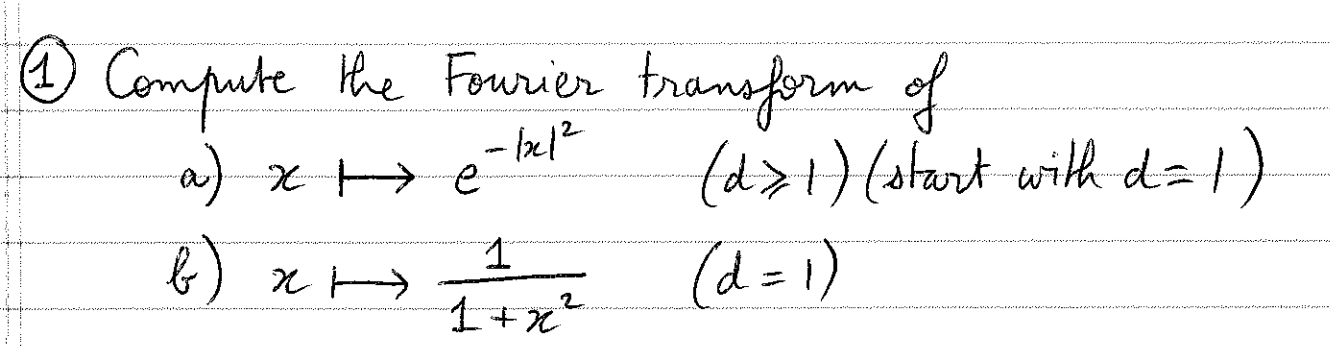
\includegraphics[width=0.7\textwidth]{pde2-1-1.png}
\end{figure}
\end{question}
\begin{solution} \hfill \\

\textbf{(a)} Set $u = x^2$ and $du = 2x dx$. Then,
\eQnb
\int_{-\infty}^{\infty} e^{-x^2} &=& \int_{0}^{\infty} u^{-\frac{1}{2}} e^{-u} du
= \Gamma(\dfrac{1}{2}). \label{eq:1-1-1}
\eQne
As
\eQb
\Gamma(1-s)\Gamma(s) &=& \dfrac{\pi}{\sin(\pi s)} 
\eQe
for any $s \in \mathbb{C}$, setting $s = \dfrac{1}{2}$ in the above and substituting
to~\eqref{eq:1-1-1} gives
\eQnb
\int_{-\infty}^{\infty} e^{-x^2} &=& \sqrt{\pi}. \label{eq:1-1-2}
\eQne
We now compute
\eQnb
\hat{f}(\xi) &=& \dfrac{1}{(2\pi)^{\frac{d}{2}}} \int_{\mathbb{R}^d} e^{-ix\cdot \xi}
e^{-|x|^2} \nonumber \\
&=& \dfrac{1}{(2\pi)^{\frac{d}{2}}} \prod_{k=1}^{d} \int_{\mathbb{R}} 
e^{-(x_k + \frac{i\xi_k}{2})^2 - \frac{\xi_k^2}{4}} dx_k \nonumber \\
&=& \dfrac{1}{(2\pi)^{\frac{d}{2}}} (\sqrt{\pi})^d e^{-\frac{|\xi|^2}{4}} 
\label{eq:1-1-3} \\ 
&=& 2^{-\frac{d}{2}}e^{-\frac{|xi|^2}{4}} \nonumber  
\eQne
for any $\xi \in \mathbb{R}^d$, where~\eqref{eq:1-1-3} follows from ~\eqref{eq:1-1-2}. 

\bigskip

\noindent 
\textbf{(b)} Firstly,
\eQnb
\hat{f}(\xi) &=& \dfrac{1}{\sqrt{2\pi}} \int_{\mathbb{R}} e^{-ix\xi} 
\dfrac{1}{1+x^2} dx \label{eq:1-2-1}
\eQne
for all $\xi \in \mathbb{R}$. Let $\xi < 0$. By Residue theroem,
\eQb
\int_{H + C_R} \dfrac{e^{-iz\xi}}{1+z^2} dz = 2\pi i \text{Res}(
\dfrac{e^{-iz\xi}}{1+z^2};i) = \pi e^{\xi}  
\eQe
for all $R > 0$ sufficiently large, where $C_R$ is the standard arc  and $H$
is the horizontal part of the upper half circle, oriented counter-clockwise. As
\eQb
\left| \int_{C_R} \dfrac{e^{-iz\xi}}{1+z^2} dz \right| &\leq& \dfrac{R}{R^2-1}
\int_{0}^{\pi} e^{R \xi \sin(\theta)} d\theta \leq \dfrac{\pi R}{R^2 -1} 
\eQe
for all $R > 0$, taking $R \to \infty$ gives
\eQb
\int_{\mathbb{R}} e^{-ix\xi} \dfrac{1}{1+x^2} dx &=& \pi e^{\xi}.
\eQe
Similarly, for $\xi \geq 0$, considering the lower half circle containing $-i$ gives
\eQb
\int_{\mathbb{R}} e^{-ix\xi} \dfrac{1}{1+x^2} dx &=& \pi e^{-\xi}
\eQe 
and hence, by~\eqref{eq:1-2-1},
\eQb
\hat{f}(\xi) &=& \sqrt{\dfrac{\pi}{2}} e^{-|\xi|} 
\eQe 
for all $\xi \in \mathbb{R}$. \hfill $\qed$ 
 
\end{solution}

\newpage

\begin{question}[1-2]
\hfill
\begin{figure}[h!]
  \centering
    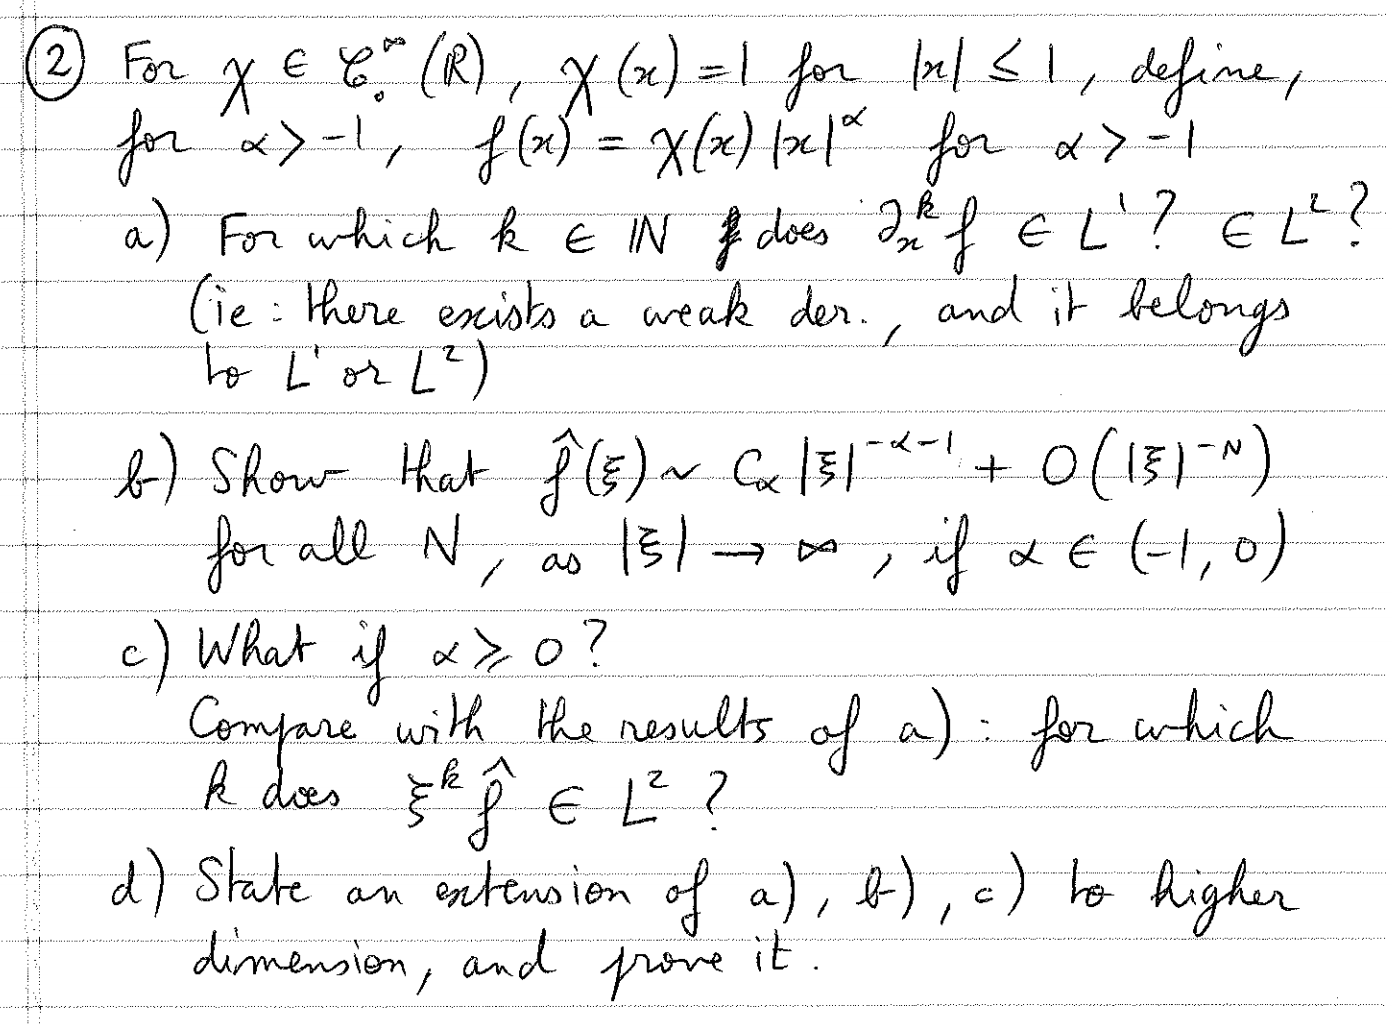
\includegraphics[width=0.7\textwidth]{pde2-1-2.png}
\end{figure}
\end{question}
\begin{solution} \hfill \\
Now, consider $\alpha \in \mathbb{Z}_+$. For $\alpha$ even, we see
\eQb
f(x) &=& X(x)|x|^{\alpha} = X(x)x^{\alpha} \in C_{0}^{\infty}(\mathbb{R}).
\eQe
Thus, $\partial_x^{k}f \in L^1 \cap L^2$ for all $k \in \mathbb{Z}_+$. For
$\alpha$ odd, as $f \in C^{\alpha-1}$, and $f^{(\alpha-1)}$ has $\text{sgn}(x)
(\alpha-1)!$
on $[-1,1]$ as weak-derivative, which we know does not have a weak derivative,
$\partial_{x}^k f \in L^1 \cap L^2$ for any $k \leq \alpha$. 

\bigskip \noindent Now, let $-1 < \alpha < 0$. Then, if $f$
has a weak-derivative, then,  for any $\phi \in \mathscr{S}$,
and $\epsilon > 0$,
\eQnb
\int_{\mathbb{R}} X(x)|x|^{\alpha} \phi^{'}(x) dx &=& \int_{\epsilon}^{\infty}
+ \int_{0}^{\epsilon} + \int_{-\epsilon}^{0} + \int_{-\infty}^{-\epsilon} 
X(x)x^{\alpha}\phi^{'}(x) dx \nonumber \\
&=& \epsilon^{\alpha}(\phi(-\epsilon) - \phi(\epsilon)) + \int_{0}^{\epsilon} +
\int_{-\epsilon}^{0} - \int_{|x| > \epsilon} g(x) \phi(x) dx \label{eq:1-2-1} 
\eQne 
where~\eqref{eq:1-2-1} holds by integration by parts, and 
\eQb
g(x) = X'(x)|X|^{\alpha} + \text{sgn}(x) \alpha X(x) |x|^{\alpha - 1}. 
\eQe
Therefore, as $g \not\in L^1_{\text{loc}}$, and $P.V_{|x|>\epsilon} g(x)$
is not a function, $\partial_x^{k} f \in L^1 \iff k = 0$, and $\partial_x^k f
\in L^2 \iff k = 0 \>\>\> \text{and} \>\>\> \alpha > - \dfrac{1}{2}$. 

\bigskip \noindent Now, consider $\alpha \geq 0$ and $\alpha \not\in \mathbb{Z}$.
Observe that $X(x)|x|^{\alpha} \in C^{\lceil \alpha \rceil}$ and 
\eQb
(X(x)|x|^{\alpha})^{\lceil \alpha \rceil} &=& \binom{\alpha}{\lfloor \alpha \rfloor}
\lfloor \alpha \rfloor ! (\text{sgn}(x))^{\lfloor x \rfloor} |x|^{\alpha - \lfloor
\alpha \rfloor} \>\>\> \text{on} \>\>\> [0,1].
\eQe
Now, for any $\phi \in \mathscr{S}$ and $\epsilon > 0$, 
\eQb
\int_{\mathbb{R}} f^{(\lfloor \alpha \rfloor)}(x) \phi^{'}(x) dx 
&=& -f^{(\lfloor \alpha \rfloor)}(x)\phi(x)|^{-\epsilon}_{\epsilon} +
\binom{\alpha}{\lfloor \alpha \rfloor}\lfloor \alpha \rfloor!(\text{sgn}(x))^{
\lfloor \alpha \rfloor} \\
&& \int_{-\epsilon}^{\epsilon}|x|^{\alpha - \lfloor \alpha 
\rfloor} \phi^{']}(x) dx - \int_{|x| > \epsilon} \phi(x) g(x) \to 
\int_{\mathbb{R}} \phi(x) g(x) dx \>\>\> \text{as} \>\>\> \epsilon \to 0^{+}
\eQe
where $g(x) = h(x) |x|^{\alpha - \lfloor \alpha \rfloor - 1}$ on $[-1,1]$
for some $h$ smooth and compactly supported. Therefore, by the above discussion,
$f$ only has weak derivative upto $\lfloor \alpha \rfloor$, and
$\partial_x^k f \in L^1$ for $k = 0,1..., \lfloor \alpha \rfloor$ and
$\partial_x^k f \in L^2$ for $k = 0,...,\lceil \alpha \rceil$ for $(\alpha) \leq 
\dfrac{1}{2}$ and $k = 0,...,\lfloor \alpha \rfloor$ for $(\alpha) > \dfrac{1}{2}$.

\bigskip \noindent \textbf{(b)} We compute 
\eQnb
\widehat{|x|^{\alpha}}(\xi) &=& \dfrac{1}{\sqrt{2\pi}} \int_{\mathbb{R}} |x|^{\alpha}
e^{-ix\xi} dx = \dfrac{1}{\sqrt{2\pi}} \int_{\mathbb{R}} |y|^{\alpha} |\xi|^{-\alpha - 1}
e^{-iy} dy \label{eq:1-2-1} \\
&=&
\dfrac{1}{\sqrt{2\pi}} \int_{\mathbb{R}} |y|^{\alpha} e^{-iy} dy  |\xi|^{-\alpha - 1}
=: C_{\alpha} |\xi|^{-\alpha - 1}  
\nonumber 
\eQne
where~\eqref{eq:1-2-1} holds by a change of variable of $y = x\xi$. Set
$g(x) = f - |x|^{\alpha} = (X(x) - 1)|x|^{\alpha}$, so
\eQb
\hat{g}(\xi) &=& \widehat{f-|x|^{\alpha}}(\xi) = \hat{f}(\xi) - C_{\alpha}|\xi|^{
-\alpha-1}.
\eQe
Since
\eQb
\partial_x^{N} g &=& \sum_{k=0}^{N} \binom{N}{k} (X(x) - 1)^{(N-k)} 
\binom{\alpha}{k} k!\text{sgn}(x)^k |x|^{\alpha - k} 
\eQe
for any $N$, we have
\eQb
|| |\xi|^{N} \hat{g}||_{L^{\infty}} &\leq& C||\partial_{x}^{N}g||_{L^1} < \infty
\eQe
and hence
\eQb
\hat{f}(\xi) &\sim& C_{\alpha}|\xi|^{-\alpha - 1} + O(|\xi|^{-N})
\eQe
for any $N$. 

\bigskip \noindent \textbf{(c)} Let $\alpha \not\in \mathbb{Z}$. Then, $f$
has weak derivative up to $\lceil \alpha \rceil$.
\eQb
\partial_{x}^{\lceil \alpha \rceil}f(x) &=& \sum_{k=0}^{\lceil \alpha \rceil -1}
X(x)^{\lceil \alpha \rceil - k}(x) \binom{\alpha}{k} k! |x|^{\alpha - k} 
(\text{sgn}x)^k\binom{\lceil \alpha \rceil}{k} + C X(x)|x|^{\alpha - \lceil x 
\rceil}. 
\eQe
Now, by (b), 
\eQb
\widehat{\partial_{x}^{\lceil \alpha \rceil}f }(\xi) &\sim& 
C_{\alpha} |\xi|^{-1 \lceil \alpha \rceil - \alpha} + O(|\xi|^{-N})  
\eQe
so 
\eQb
\hat{f}(\xi) &\sim& C_{\alpha}|\xi|^{-1-\alpha} + O(|\xi|^{-N}) 
\eQe
and hence $|\xi|^k \hat{f} \in  L^2$ iff $k -1 - \alpha < -\dfrac{1}{2}$. Now,
for $\alpha$ even, if $f \in C^{\infty}_0(\mathbb{R})$, then 
$|||\xi|^N \hat{f}||_{\infty} \leq C |||\partial_x^{N} f||_{L^1} < \infty$, so
$\hat{f} \sim O(|\xi|^{-N})$ for all $N$, and $|\xi|^k \hat{f} \in L^2$ for all $k$. 

\bigskip

\noindent 
For $\alpha$ even, if $f \in C_{0}^{\infty}(\mathbb{R})$, then 
$||\xi|^N \hat{f}||_{\infty} \leq C ||\partial_x^{N} f||_{L^1} < \infty$, so 
$\hat{f} \sim O(|\xi|^{-N})$ for all $N$, and $|\xi|^k\hat{f} \in L^2$ for all $k$.

\bigskip

\noindent
For $\alpha$ odd, we have that $f$ has weak derivative only up to order $\alpha$. So,
$|||\xi|^{N} \hat{f}||_{L^1} \leq C ||\partial_x^{N} f||_{L^1} < \infty$, and
$\hat{f}(\xi) \sim O(|\xi|^{-N})$ for $N \leq \alpha + 1$. Therefore, $|\xi|^k \hat{f} 
\in L^2$ for $k \leq \alpha$.  

\bigskip

\noindent \textbf{(d)} The proof does not change for higher dimension from the first
parts.

\bigskip

\noindent a) For $\alpha$ odd, $\partial_x^{k} f \in L^1 \cap L^2$
for all $k \leq \alpha$. For $\alpha$ even, $\partial_x^{k} f \in L^1 \cap L^2$
for all $k$. For $\alpha \not \in \mathbb{Z}$, if $k < \alpha + \dfrac{d}{2}$, 
$|\xi|^k \hat{f} \in L^2 \implies \partial_x^{k} f \in L^2 \implies \partial_x^{k} f
\in L^1$. 

\bigskip

\noindent
b) $\alpha \in (-d,0)$, $\hat{f}(\xi) \sim C_{\alpha}|\xi|^{-\alpha - d} + 
O(|\xi|^{-N})$ for all $N$.

\bigskip
\noindent 
c) $\alpha \not\in \mathbb{Z}$. If $\alpha + \dfrac{d}{2} > k$, then, 
$\hat{f}(\xi) \sim C_{\alpha} |\xi|^{-\alpha - d} + O(|\xi|^{-N})$ and $|\xi|^k\hat{f}
\in L^2$. $\alpha$ even is the same. For $\alpha$ odd, 
$\hat{f} \sim O(|\xi|^{-\alpha - d})$ and $|\xi|^k\hat{f} \in L^2$ for $k < 
\alpha + \dfrac{d}{2}$.  

\end{solution}

\newpage

\begin{question}[1-3]
\hfill
\begin{figure}[h!]
  \centering
    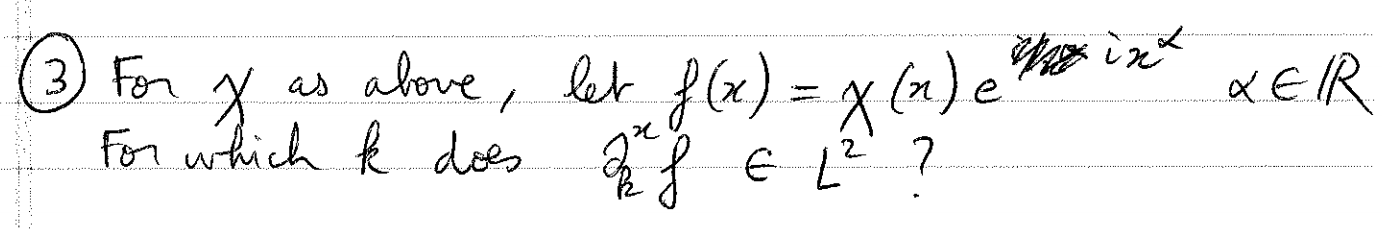
\includegraphics[width=0.7\textwidth]{pde2-1-3.png}
\end{figure}
\end{question}
\begin{solution} \hfill \\
By the same line of reasoning as above, for $\alpha \in \mathbb{Z}$,
$\partial_{x}^k f \in L^2$ for all $k \in \mathbb{Z}_+$. Let $\alpha \not\in 
\mathbb{Z}$. Integrating by parts, for any $\phi \in \mathscr{S}$, and $\epsilon > 0$,
\eQb
\int_{\mathbb{R}} X(x)e^{ix^{\alpha}} \phi^{'}(x) dx &=& -X(x)e^{ix^{\alpha}}
\phi(x)|_{-\epsilon}^{\epsilon} + \int_{-\epsilon}^{\epsilon} X(x)e^{ix^{\alpha}} 
\phi(x) dx - \int_{|x|>\epsilon} \phi(x) g(x) dx 
\eQe 
where
\eQb
g(x) &=& X'(x)e^{ix^{\alpha}} + \text{sgn}(x) i\alpha X(x) x^{\alpha - 1} e^{ix^{\alpha}} 
\eQe 
for $x \in \mathbb{R}$. Taking $\epsilon \to 0^{+}$ $f' \sim x^{\alpha - 1}$, and 
similarly $f^{(k)} \sim x^{\alpha - k}$. Therefore, $\partial_x^{k}f \in L^2
\iff 2\alpha - 2k > -1$ and $\alpha + \dfrac{1}{2} > k$. \hfill $\qed$  

\end{solution}

\newpage

\begin{question}[1-4]
\hfill
\begin{figure}[h!]
  \centering
    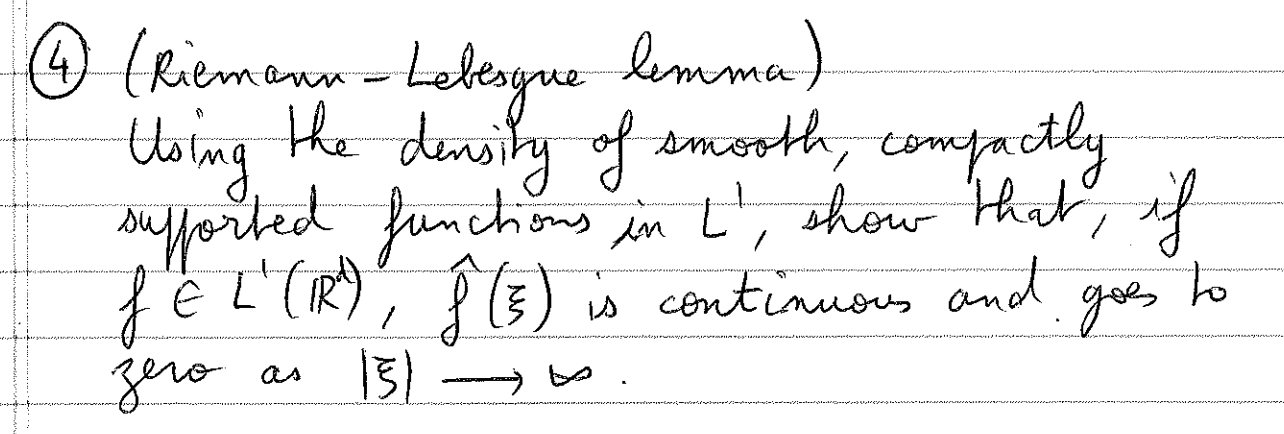
\includegraphics[width=0.7\textwidth]{pde2-1-4.png}
\end{figure}
\end{question}
\begin{solution} \hfill \\
The key property in this problem is that smooth and compactly supported functions
on $\mathbb{R}^d$ are dense in $L^1(\mathbb{R}^d)$, and $L^1$ convergence gives
uniform control on the Fourier domain.

\bigskip

\noindent
Let $f \in L^1(\mathbb{R}^d), \xi \in \mathbb{R}^d$. Then, 
\eQb
|\hat{f}(\xi + \delta) - \hat{f}(\xi)| &=& \left|
\dfrac{1}{(2\pi)^{\frac{d}{2}}} \int_{\mathbb{R}^d} e^{-i x \cdot (\xi+\delta) } 
f(x) dx-
\dfrac{1}{(2\pi)^{\frac{d}{2}}} \int_{\mathbb{R}^{d}}  e^{-i x \cdot \xi} f(x) dx \right|
\\
&\leq& \dfrac{1}{(2\pi)^{\frac{d}{2}}} \int_{\mathbb{R}^d} |f(x)||e^{-ix \cdot 
(\xi+\delta)} - e^{-ix \cdot \xi}| dx \\
&\leq& \dfrac{1}{(2\pi)^{\frac{d}{2}}} \int_{\mathbb{R}^d} 2|f(x)| dx \in 
L^1(\mathbb{R}^d) 
\eQe
for all $\delta \in \mathbb{R}^d$. As 
\eQb
|e^{-ix \cdot (\xi + \delta)} - e^{-ix \cdot \xi} | \to 0 \>\>\> \text{as} 
\>\>\> \delta \to 0
\eQe
for all $x \in \mathbb{R}^d$, by DCT,
\eQb
\dfrac{1}{(2\pi)^{\frac{d}{2}}} \int_{\mathbb{R}^d} |f(x)||e^{-ix \cdot 
(\xi+\delta)} - e^{-ix \cdot \xi}| dx \to 0 \>\>\> \text{as} \>\>\> \delta \to 0 \\
\eQe
and hence, 
\eQb
\lim_{\delta \to 0} \hat{f}(\xi + \delta) - \hat{f}(\xi) &=& 0, 
\eQe
which shows that $\hat{f}$ is continuous.

\bigskip

\noindent Let $f \in C_{0}^{\infty}(\mathbb{R}^d)$ and $\xi \in \mathbb{R}^d$. Then, 
\eQnb
|\hat{f}(\xi)| &=& \left| \dfrac{1}{{(2\pi)}^{\frac{d}{2}}} 
\int_{\mathbb{R}^d}e^{-ix\cdot \xi} f(x) dx \right| 
= \left| - \dfrac{1}{(2\pi)^{\frac{d}{2}}} \int_{\mathbb{R}^d} 
\triangledown f(x) \cdot \triangledown (\frac{e^{ix\cdot \xi}}{-|\xi|^2}) \right| 
\label{eq:1-4-1} \\
&\leq& \dfrac{1}{(2\pi)^{\frac{d}{2}} |\xi|^2}  \int_{\mathbb{R}^d} 
\left| \triangledown 
f(x) \cdot (-i\xi e^{-ix\cdot \xi}) \right| dx \leq
\dfrac{1}{(2\pi)^{\frac{d}{2}} |\xi|^2}  \int_{\mathbb{R}^d} 
\left| \triangledown f(x) \cdot \xi \right| dx \nonumber \\
&\leq& \dfrac{1}{(2\pi)^{\frac{d}{2}}|\xi|^2} 
\sum_{i=1}^{d}|\xi_i| \int_{\mathbb{R^d}}|
f_i(x)| dx 
\leq \dfrac{1}{(2\pi)^{\frac{d}{2}}|\xi|^2} \max_{i \leq d} |\xi_i| 
\sum_{i \leq d} \int_{\mathbb{R}^d} |f_i(x)| dx \nonumber \\
&\lesssim& \dfrac{1}{|\xi|} \max_{i \leq d}  ||f_i||_{L_1} \label{eq:1-4-2} 
\eQne 
where~\eqref{eq:1-4-1} holds by integration by parts, and~\eqref{eq:1-4-2} holds
by the topological 
equivalence of the norms in $\mathbb{R}^d$. By the compactness assumption, 
taking $|\xi| \to \infty$ sends RHS to $0$. Therefore, 
the Riemann-Lebesgue lemma holds for $f \in C_{0}^{\infty}(\mathbb{R}^d)$.
Now, suppose $f \in L^1(\mathbb{R}^d)$. Then, by density of $C_0^{\infty}(\mathbb{R}^d)$
in $L^1(\mathbb{R}^d)$, 
we can choose $\{f_n\}_{n \in \mathbb{N}} 
\subset C_0^{\infty}(\mathbb{R}^d)$ such that $f_n \to_{L^1} f$ as $n \to \infty$.
Observe that there is some $C > 0$ such that for all $\xi \in \mathbb{R}^d$ and $n \in 
\mathbb{N}$, 
\eQb
|\hat{f}(\xi) - \hat{f_n}(\xi)| &\leq& C||f_n - f|| 
\eQe
and hence $\hat{f_n}$ converges uniformly to $\hat{f}$. Fix $\epsilon > 0$.
Then, we can choose $f_n$ such that $||\hat{f_n} - \hat{f}||_{\infty} <
\frac{\epsilon}{2}$ and choose $M$ large enough that $|\hat{f}_n(\xi)| < \frac{
\epsilon}{2}$ for all $\xi$ such that $|\xi| > M$. Therefore, for any $\xi$ with
$|\xi| > M$, $|\hat{f}(\xi)| < \epsilon$, so 
\eQb
\hat{f}(\xi) \to 0 \>\>\> \text{as} |\xi| \to \infty,
\eQe 
as required. \hfill $\qed$

\end{solution}

\newpage

\begin{question}[1-5]
\hfill
\begin{figure}[h!]
  \centering
    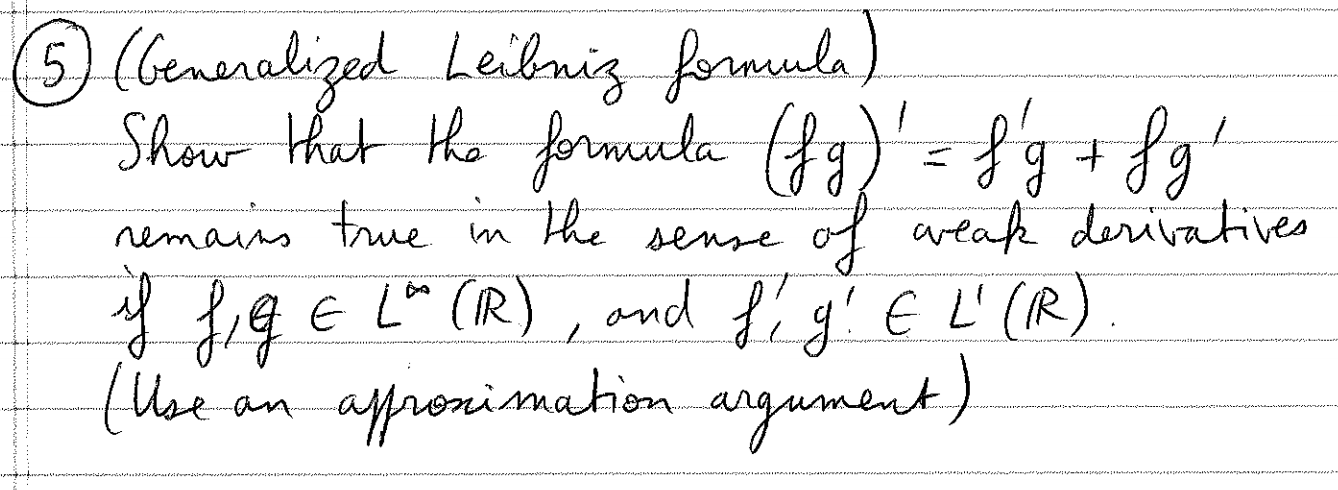
\includegraphics[width=0.7\textwidth]{pde2-1-5.png}
\end{figure}
\end{question}
\begin{solution} \hfill \\
Consider an approximate identity $\{\phi_{\epsilon}\}_{\epsilon > 0} \subset
C_{0}^{\infty}$. Then,
\eQb
(\phi_{\epsilon} * f)^{'}(x) &=& \int_{\mathbb{R}} \phi_{\epsilon}^{'}(x-y)
= -(-1) \int_{\mathbb{R}} \phi_{\epsilon}(x-y)f^{'}(y) dy = \phi_{\epsilon} * f'  
\eQe
for any $x \in \mathbb{R}, \epsilon > 0$, so $(\phi_{\epsilon}* f)^{'} =
\phi_{\epsilon} * f'$. Similarly, $(\phi_{\epsilon} * g)^{'}
= \phi_{\epsilon} * g'$. Furthermore, by a property of approximate identity
\eQb
\phi_{\epsilon} *g' \to_{L^1} g' \>\>\> &\text{and}& \>\>\> \phi_{\epsilon} * f' 
\to_{L^1} f'.
\eQe
Now, for any $\phi \in \mathscr{S}$, and $\epsilon > 0$,
\eQb
\int_{\mathbb{R}} (\phi_{\epsilon} * f \phi_{\epsilon} * g) \phi^{'} dx
&=& \int_{\mathbb{R}} (\phi_{\epsilon} * f \phi_{\epsilon} *g)' \phi dx 
\label{eq:1-5-1} \\
&=& \int_{\mathbb{R}} (\phi_{\epsilon} * f' \phi_{\epsilon} *g + 
\phi_{\epsilon}*g' \phi_{\epsilon}*f) \phi dx \nonumber 
\eQe
where~\eqref{eq:1-5-1} holds by $\phi_{\epsilon} * f, \phi_{\epsilon} * g
\in C_{0}^{\infty}$. Taking $\epsilon \to 0$, by DCT,
\eQb
\int_{\mathbb{R}} fg \phi^{'} &=& \int_{\mathbb{R}} (f'g + g'f)\phi
\eQe
for all $\phi \in \mathscr{S}$, so $(fg)' = f'g + fg'$ as required. \hfill $\qed$ 
\end{solution}


\end{document}
